%!TEX root = M1P1.tex

\stepcounter{lecture}

\pagebreak
\setcounter{section}{-1}

\setcounter{lecture}{0}

\setcounter{page}{4}
\sektion{Preliminaries}
\lecturemarker{1}{5 Oct}


M1F stuff:

\begin{itemize}
\item $\forall - \text{ for any, \textbf{fix any}, for all, every...}$
\item $\exists - \text{ there exists}$
\item $\mathbb{N} = \{1,2,3,\dots\}$ 
\end{itemize}

\begin{theorem}[Triangle Inequality]
(See Question Sheet 1)
	\[|a+b| \leq |a| + |b|\]
\end{theorem}

\begin{corollary}
\[\left||a| - |b|\right|\leq |a-b|	\]
\end{corollary}
\begin{proof}
\[
\begin{aligned}
|a-b| < \epsilon &\iff b-\epsilon < a < b + \epsilon\\
&\iff a \in (b-\epsilon, b+\epsilon)\\
&\iff b \in (a-\epsilon, a+\epsilon)	\\
&\implies \left||a| - |b|\right|< \epsilon
\end{aligned} \] 
\end{proof}

Lots of other versions, see Question Sheet 1 - \emph{don't try to memorise them!}\\



\begin{clicker}
Fix $a \in \mathbb{R}$. What does the statement 
\[\forall \epsilon >0,~|x-a|<\epsilon ~(*)\]
mean for the number $x$? 

\textbf{Answer:} $x = a$. 
\begin{proof}
Assume $x \neq a$. Take $\epsilon := \frac{1}{2}|x-a| > 0$. Then $(*)$ does not hold.	
\end{proof}

\end{clicker}







\stepcounter{lecture}
\setcounter{lecture}{1}

\sektion{Sequences}
\lecturemarker{2}{5 Oct}
\label{sub:sequences}

A sequence $(a_n)_{n\geq 1}$ of real (or complex, etc.) numbers is an infinite list of numbers $a_1,~a_2,~a_3,\dots$ all in $\mathbb{R}$ (or $\mathbb{C}$, etc.) Formally:\\

\begin{definition}
	A \emph{sequence} is a function $a:\mathbb{N} \to \mathbb{R}$
\end{definition}

\textbf{Notation:} We let $a_n \in \mathbb{R}$ denote $a(n)$ for $n \in \mathbb{N}$. The data $(a_n)_{n=1,2,\dots}$ is equivalent to the function $a:\mathbb{N} \to \mathbb{R}$ because a function $a$ is determined by its values $a_n$ over all $n \in \mathbb{N}$. 

We will denote $a$ by $a_1,~a_2,\dots$ or $(a_n)_{n\in\mathbb{N}}$ or $(a_n)_{n\geq 1}$ or even just $(a_n)$.

\begin{remark}
$a_i$'s could be repeated, so $(a_n)$ is \emph{not} equivalent to the set $\{a_n : n \in \mathbb{N}\}\subset \mathbb{R}$. E.g. $(a_n) = 1,~0,~1,~0,\dots$ is different from $(b_n) = 1,~0,~0,~1,~0,~0,~1,\dots$	
\end{remark}

We can describe a sequence in may ways, e.g. formula for $a_n$ as above $a_n = \frac{1-(-1)^n}{2}$, or a recursion e.g. $c_1 = 1 = c_2$, $c_n = c_{n-1} + c_{n-2}$ for $n\geq 3$, or a summation (see next section) e.g. $d_n = \sum_{i=1}^n \frac{1}{i} = 1 + \frac{1}{2} + \frac{1}{3} + \dots +\frac{1}{n}$.

\subsektion{Convergence of Sequences}
We want to \emph{rigorously} define $a_n \to a \in \mathbb{R}$, or ``$a_n$ converges to $a$ as $n \to \infty$" or ``$a$ is the limit of $(a_n)$". 

Idea: $a_n$ should get closer and closer to $a$. Not necessarily monotonically, e.g.:
\[a_n = 
\begin{cases}
\frac{1}{n} & n \text{ odd}\\
\frac{1}{2n} & n \text{ even}	
\end{cases}
\hspace*{20pt}\text{ we want } a_n \to 0\]


\begin{center}
\begin{tikzpicture}
\begin{axis}[axis lines=middle,
     x label style={at={(axis description cs:0.95,-0.15)}},
     y label style={at={(axis description cs:-0.1,0.9)}},
    xlabel={$n$},
    ylabel={$a_n$},
    ticks=none,
  ymin = 0,
  ymax = 0.4,
  xmin = 1,
  xmax = 10,
  width=10cm,height=5cm]
   \addplot[samples at={3,5,7,9}, only marks, mark=x, mark size=3pt]{1/x};
    \addplot[samples at={2,4,6,8},only marks,mark=x,mark size=3pt]{(1/(2*x))};
  \end{axis}
\end{tikzpicture}
\end{center}
Also notice that $\frac{1}{n}$ gets closer and closer to $-1$! So we want to say instead that $a_n$ gets \emph{as close as we like to $a$}. We will measure this with $\epsilon >0$. We phrase ``$a_n$ gets \emph{arbitrarily} close to $a$" by ``$a_n$ gets to within $\epsilon$ of $a$ for \emph{any} $\epsilon >0$".\\

\begin{definition}[Mestel]
	$u_n \to u$ if $\forall n$ sufficiently large, $|u_n - u|$ is \emph{arbitrarily small.} 
	
Define a real number $b \in \mathbb{R}$ to be arbitrarily small if it is smaller than any $\epsilon >0$ i.e. $\forall \epsilon >0,~|b| < \epsilon$.
\end{definition}

Definition Mestel says that once $n$ is large enough, $|u_n - u|$ is less than every $\epsilon >0$, i..e it's zero, i.e. $u_n = u$. We want to \emph{reverse} the order of specifying $n$ and $\epsilon$. 

i.e. we want to say that to get \emph{arbitrarily close to the limit $a$} (i.e. $|a_n - a| < \epsilon$), we need to go sufficiently far down the sequence. Then if I change $\epsilon >0$ to be smaller, I simply go further down the sequence to get within $\epsilon$ of $a$. 

\begin{center}
\begin{tikzpicture}
\begin{axis}[
 axis line style={red},
axis lines=middle,
     x label style={at={(axis description cs:1.05,0.33)}},
     y label style={at={(axis description cs:-0.1,1.1)}},
    xlabel={\small $n$},
    ylabel={$a_n \to 0$},
  ymin = -0.4,
  ymax = 0.7,
  xmin = 1,
  xmax = 20,
    ytick = {0.3,0.12},
   yticklabels={$\epsilon_1$,$\epsilon_2$},
   xtick = 0,
  width=12cm,height=8cm]
   \addplot[samples at={2,...,20}, only marks, mark=x, mark size=2pt,  mark options={red},]{1/x};
   \draw (axis cs:20,0.3) -- (axis cs:0,0.3);
      \draw (axis cs:20,0.12) -- (axis cs:0,0.12);
     \draw (axis cs:20,-.1) -- (axis cs:4,-.1) node at (axis cs:10,-0.15){\small $n$ suff. large for $|a_n - 0| < \epsilon_1$};
          \draw (axis cs:4,-.06) -- (axis cs:4,-.1);
          \draw (axis cs:20,-.06) -- (axis cs:20,-.1);
          \draw (axis cs:20,-.25) -- (axis cs:9,-.25) node at (axis cs:15,-0.3){\small $n$ suff. large for $|a_n - 0| < \epsilon_2$};
           \draw (axis cs:9,-.2) -- (axis cs:9,-.25);
          \draw (axis cs:20,-.2) -- (axis cs:20,-.25);

  \end{axis}
\end{tikzpicture}
\end{center}

There will not be a ``$n$ sufficiently large" that works for all $\epsilon$ at once! (unless $a_n = a$ eventually.)

But for \emph{any} (fixed) $\epsilon>0$ we want there to be an $n$ sufficiently large such that $|a_n - a| < \epsilon$. So we change ``$\exists n$ such that $\forall \epsilon$" to ``$\forall \epsilon,~\exists n.$". \emph{This allows $n$ to depend on $\epsilon$.}~\\

\begin{definition}[Nestel]
	$a_n \to a$ if $\forall \epsilon >0,~\exists n \in \mathbb{N}$ such that $|a_n - a| < \epsilon$. 
\end{definition}

e.g. 
\[
a_n = \begin{cases}
 0 & n\text{ even}\\
 1 & n\text{ odd}	
 \end{cases}
 \text{ satisfies } a_n \to 0 \text{ according to Prof. Nestel.}
\]

We want to modify this to say eventually $|a_n - a| < \epsilon$ \emph{and it stays there!}\vspace*{5pt}

\textbf{Ignore Mestel and Nestel's definition!}\lecturemarker{3}{5 Oct}\\

\begin{definition}[Convergence]
We say that $a_n \to a$ iff 
\[\forall \epsilon >0,~\exists N \in \mathbb{N} \text{ such that } ``n \geq N \implies |a_n - a| < \epsilon"\]	
\end{definition}

This says that \emph{however close} ($\forall \epsilon>0$) I want to get to the limit $a$, there's a point in the sequence ($\exists N \in \mathbb{N}$) beyond which ($n \geq N$) my $a_n$ is indeed that close to the limit $a$ ($|a_n - a| <\epsilon$).\\ 

\begin{remark}
$N$ depends on $\epsilon$! $N = N(\epsilon)$	
\end{remark}

Equivalently:
\[\forall \epsilon >0,~ \exists N \in \mathbb{N} \text{ such that} ``\forall n \geq N,~|a_n -a|<\epsilon"\]
or equivalently
\[\forall \epsilon >0,~\exists N_\epsilon\in\mathbb{N} \text{ such that } |a_n - a| < \epsilon,~\forall n \geq N_\epsilon\]

\begin{clicker}Given a sequence of real numbers $(a_n)_{n\geq 1}$. Conisder 
\[\boxed{\forall n \geq 1,~\exists \epsilon >0 \text{ such that } |a_n|< \epsilon}\]
This means? 

\textbf{Answer:} It always holds. \begin{proof}
 Fix any $n \in \mathbb{N}$. Take $\epsilon = |a_n| + 1$. 	
 \end{proof}
 
What about
 \[\boxed{\exists \epsilon >0 \text{ such that } \forall n \geq 1,~|a_n| < \epsilon} \]
 
 \textbf{Answer:} $(a_n)$ is bounded.
 
 
\begin{center}
\begin{tikzpicture}
\begin{axis}[
 axis line style={red},
axis lines=middle,
     x label style={at={(axis description cs:1.05,0.4)}},
     y label style={at={(axis description cs:-0.1,1.1)}},
    xlabel={\small $n$},
    ylabel={$a_n$},
  ymin = -0.4,
  ymax = 0.4,
  xmin = 1,
  xmax = 10,
     ytick = {0.3, -.3},
   yticklabels={$\epsilon$,$-\epsilon$},
   xtick = 0,
  width=10cm,height=5cm]
   \addplot[samples at={5,7,9}, only marks, mark=x,  mark options={red}, mark size=3pt]{(-1)^x*1/x};
    \addplot[samples at={2,3,4,6,8},only marks, mark options={red},mark=x,mark size=3pt]{(1/(2*x))};
       \draw (axis cs:20,0.3) -- (axis cs:0,0.3);
      \draw (axis cs:20,-0.3) -- (axis cs:0,-0.3);
  \end{axis}
\end{tikzpicture}
\end{center}


  \begin{proof}
$\iff a_n \in (-\epsilon,\epsilon)~ \forall n \iff |a_n|$ is bounded by $\epsilon$. \end{proof}

\end{clicker}~

\begin{definition}
If $a_n$ does not converge to $a$ for any $a\in \mathbb{R}$, we say that $a_n$ \emph{diverges.}
\end{definition}~

\begin{example}
I claim that $\frac{1}{n} \to 0$ as $n \to \infty$

\textit{Rough working:} Fix $\epsilon >0$. I want to find $N \in \mathbb{N}$ such that $|a_n - a| = |\frac{1}{n} - 0| = \frac{1}{n} < \epsilon$ for all $n \geq N$. 
\begin{center}
\begin{tikzpicture}
\begin{axis}[
 axis line style={red},
axis lines=middle,
     x label style={at={(axis description cs:1.05,0.1)}},
     y label style={at={(axis description cs:-0.1,1.1)}},
    xlabel={\small $n$},
    ylabel={$a_n$},
  ymin = -0.1,
  ymax = 0.4,
  xmin = 1,
  xmax = 10,
     ytick = {0.15},
   yticklabels={$\epsilon$},
   xtick = 0,
  width=10cm,height=5cm]
   \addplot[samples at={5,7,9}, only marks, mark=x,  mark options={red}, mark size=3pt]{(-1)^x*1/x};
    \addplot[samples at={2,3,4,6,8},only marks, mark options={red},mark=x,mark size=3pt]{(1/(2*x))};
       \draw (axis cs:20,0.15) -- (axis cs:0,0.15);
        \draw (axis cs:4,0.12) -- (axis cs:4,-0.1) node at (axis cs:4.2,-0.05) {$N$};
  \end{axis}
\end{tikzpicture}
\end{center}


Since $a_n = \frac{1}{n}$ is monotonic, it is \emph{sufficient} to ensure that $\frac{1}{N} < \epsilon \iff N > \frac{1}{\epsilon}$ (This \emph{implies} $\frac{1}{n} \leq \frac{1}{N} < \epsilon,~\forall n \geq N$).

\begin{proof}
Fix $\epsilon >0$. 
 Pick any $N \in \mathbb{N}$ such that $N > \frac{1}{\epsilon}$. (This is the Archimedean axiom of $\mathbb{R}$. Notice $N$ depends on $\epsilon$!!). Then $n \geq N \implies |\frac{1}{n}-0| = \frac{1}{n} \leq \frac{1}{N} < \epsilon$.
\end{proof}


\end{example}


\textbf{Method to prove $a_n \to a$}
\begin{enumerate}
\item[(I)] Fix $\epsilon > 0$
\item[(II)] Calculate $|a_n - a|$
\item[(II$'$)] Find a good estimate $|a_n - a| < b_n$
\item[(III)] Try to solve $a_n - a < b_n < \epsilon ~~(*)$
\item[(IV)] Find $N \in \mathbb{N}$ s.t. $(*)$ holds whenever $n \geq N$
\item[(V)] Put everything together into a logical proof (usually involves rewriting everything in reverse order - see examples below)
\end{enumerate}~

\begin{example}
$a_n = \dfrac{n+5}{n+1}$\\

\emph{Rough Working}
\[ |a_n - 1| = \left| \dfrac{n+5}{n+1} -1 \right| = \dfrac{4}{n+1}\]

This is $< \epsilon \iff n+1 > 4/\epsilon \iff n > 4/\epsilon$, so take $N \geq 4/\epsilon$. 

\begin{proof}
Fix $\epsilon > 0$. Pick $N$ such that $N \geq 4/\epsilon$. Then $\forall n \geq N$, \[|a_n - 1| = \frac{4}{n+1} \leq \frac{4}{N+1} < \frac{4}{N} \leq \epsilon\qedhere\]
\end{proof}
\end{example}~

\begin{example}$a_n = \dfrac{n+2}{n-2} \to 1$\\

\emph{Rough Working} 
\[|a_n -1| = \left|\frac{n+2}{n-2} - 1\right| = \frac{4}{n-2}\]

We want $\frac{4}{n-2} < \epsilon$. We want implications in the $\impliedby$ direction (i.e. $\frac{4}{n-2} < \epsilon \impliedby n \geq N$) \emph{not} $\implies$ direction. i.e. $\frac{4}{n-2} < \epsilon \implies \frac{4}{n} < \epsilon$.

But if we take $N = \frac{4}{\epsilon}$, we need the \emph{opposite} implication, we \emph{need} $\frac{4}{n-2} < \epsilon$. We \emph{need} to estimate $\frac{4}{n-2} < b_n$, and then solve $b_n < \epsilon$. So we make denominator smaller. 

To make $n-2$ smaller, make $2$ bigger! e.g. $\frac{n}{2}>2$ for $n>4$. Then $\frac{4}{n-2} < \frac{4}{n-n/2} = \frac{8}{n}$

Also want $b_n = \frac{8}{n} < \epsilon \iff n > 8/\epsilon$. So take $N > \mathrm{max}(8/\epsilon, 4)$.

\begin{proof}
Fix $\epsilon > 0.$	Choose $N \iN$ such that $N > \mathrm{max}(8/\epsilon, 4)$. Then $n \geq N \implies n > 8/\epsilon~ (1)$ and $n > 4 ~(2) \implies$

\[\left|\frac{n+2}{n-2} - 1\right| = \frac{4}{n-2} \underbrace{<}_{(2)} \frac{4}{n-n/2} = \frac{8}{n} \underbrace{<}_{(1)} \epsilon\qedhere\]

\end{proof}

	
\end{example}
\pagebreak


\lecturemarker{4}{5 Oct}
We can also define limits for \emph{complex sequences}.\\

\begin{definition}
$a_n \in \mathbb{C},~\forall n \geq 1$. We say $a_n \to a \in \mathbb{C}$ iff
\[\forall \epsilon >0,~\exists N \in \mathbb{N} \text{ such that } n \geq N \implies |a_n - a| < \epsilon\]	

(i.e. $\sqrt{\Re(a_n-a)^2 + \frak{I}(a_n-a)^2} < \epsilon$) 

This is equivalent (see problem sheet!) to $(\frak{R}a_n) \to \frak{a}$ \emph{and} $(\frak{I}a_n) \to \frak{I}a$
\end{definition}~

\begin{example}
Prove $a_n = \dfrac{e^{in}}{n^3-n^2-6} \to 0$ as $n \to \infty$\\

\emph{Rough Working} 
\[|a_n - a| = \left|\dfrac{e^{in}}{n^3-n^2-6} \right| = \left|\frac{1}{n^3-n^2-6}\right|\]

\emph{Estimate} $\left|\dfrac{1}{n^3-n^2-6}\right| < \dfrac{1}{c_n}$ by making $c_n$ smaller than $n^3 - n^2 - 6$ (But not too small! We want $c_n \to \infty$). So let $c_n = n^3 - \text{\emph{ something bigger than} } n^2 + 6$.

Take off $\frac{n^3}{2}$ to make the expression simple. For $n \geq 4$, we have $\frac{n^3}{2} > n^2 + 6$. 

So for $n \geq 4$
\[\left|\frac{1}{n^3-n^2-6}\right| < \frac{1}{n^3- n^3/2} = \frac{2}{n^3} \]
and this is $< \epsilon$ for $n > \sqrt[3]{\frac{2}{\epsilon}}$.

\begin{proof}
$\forall \epsilon > 0$, choose $N \geq \mathrm{max}(4,\sqrt[3]{2/\epsilon})$	. Then $\forall n \geq N$
\[|a_n - 0| = \left| \frac{1}{n^3-n^2 - 6}\right| < \frac{1}{n^3- n^3/2} = \frac{2}{n^3} \leq \frac{2}{N^3} \leq \epsilon \qedhere \]
\end{proof}
\end{example}~


\begin{example}
Set $\delta = 10^{-1000000}, ~a_n = (-1)^n\cdot\delta$. Prove that $a_n$ does not converge. 

We want to show that the following is false: 
\[\exists a \text{ s.t. } \forall \epsilon > 0,~\exists N \in \mathbb{N} \text{ s.t. } n \geq N \implies |a_n - a| <\epsilon\]
i.e. we need to prove
\[\forall a,~ \exists \epsilon > 0 \text{ s.t. } \forall N \in \mathbb{N},~\exists n \geq N \text{ s.t. } |a_n-a| \geq \epsilon\]

\emph{Rough:} 	
Assume for contadiction that $a_n \to a$, i.e. $\forall \epsilon > 0,~\exists N \in \mathbb{N} \text{ s.t. } n \geq N \implies |a_n - a| <\epsilon$


\begin{center}
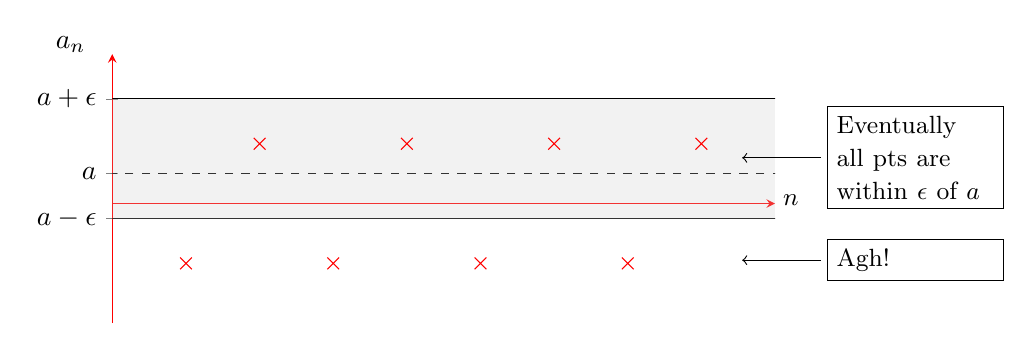
\begin{tikzpicture}
\begin{axis}[
 axis line style={red},
axis lines=middle,
     x label style={at={(axis description cs:1.05,0.4)}},
     y label style={at={(axis description cs:-0.1,1.1)}},
    xlabel={\small $n$},
    ylabel={$a_n$},
  ymin = -0.4,
  ymax = 0.5,
  xmin = 1,
  xmax = 10,
     ytick = {0.35, -0.05,0.1},
   yticklabels={$a+\epsilon$,$a-\epsilon$, $a$},
   xtick = 0,
  width=10cm,height=5cm]
   \addplot[samples at={3,5,7,9}, only marks, mark=x,  mark options={red}, mark size=3pt]{0.2};
    \addplot[samples at={2,4,6,8,},only marks, mark options={red},mark=x,mark size=3pt]{-0.2};
       \draw (axis cs:20,0.35) -- (axis cs:0,0.35); %a+e line
      \draw (axis cs:20,-0.05) -- (axis cs:0,-0.05); %a-e line
       \draw[dashed] (axis cs:20,0.1) -- (axis cs:0,0.1); %a line
         \fill[gray!40,nearly transparent] (axis cs:0,-.05)-- (axis cs: 0,0.35) -- (axis cs: 10,0.35) -- (axis cs: 10,-0.05) -- cycle;
  \end{axis}
   \draw[->] (9,2.1) -- (8,2.1);
      \draw[->] (9,0.8) -- (8,0.8);
      \node[draw,text width=2cm] at (10.2,2.1) {\small Eventually all pts are within $\epsilon$ of $a$};
        \node[draw,text width=2cm] at (10.2,0.8) {\small Agh!};
\end{tikzpicture}
\end{center}


For small enough $\epsilon >0$, the fact that $a$ is within $\epsilon$ of $\delta ~ (a_{2n})$ and $-\delta ~(a_{2n+1})$ will be a contradiction. 


\begin{proof}
Fix $a\iR$. Take $\epsilon = \delta$ (or $\epsilon < \delta$ will do). 

 Then if $\exists N$ s.t. $\forall n \geq N$, $|a_n - a| <\epsilon$ this implies
\begin{enumerate}
\item $|a_{2N} - a | < \epsilon \iff a \in (\delta - \epsilon, \delta + \epsilon)\implies a > \delta - \epsilon =0$ 
\item $|a_{2N+1} - a | < \epsilon\iff a \in (-\delta - \epsilon,-\delta + \epsilon) \implies a < -\delta + \epsilon = 0,~\cont$ 
\end{enumerate}
(or use triangle inequality: \[|\delta - (-\delta)| \leq |\delta - a| + |a -(-\delta)| < \epsilon + \epsilon \implies 2\delta < 2\epsilon = 2\delta ~\cont\text{)}\]
So $a_n \not\to a$, but this holds $\forall a \in \RR$, so $a_n$ does not converge.
\end{proof}
\end{example}~

\begin{clicker}
Fix $(a_n)_{n\geq 1},~a_n \in \RR$. Then \[\forall n,~\exists \epsilon >0 \text{ s.t. } |a_n| < \epsilon \text{ means?}\]

\textbf{Answer:} Nothing. This is always true. Take $\epsilon = |a_n| + 1$	
\end{clicker}~

\lecturemarker{5}{5 Oct}

\begin{theorem}[Uniqueness of Limits]
Limits are unique. If $a_n \to a$ and $a_n \to b$, then $a=b$	
\end{theorem}

\emph{Idea:} For $n$ large, $a_n$ should be close to $a$ and to $b$. So $a$ arbitrarily close to $b \implies a = b$. 

\begin{proof}[Proof 1]~
\begin{enumerate}
\item $\forall \epsilon,~\exists N_a$ s.t. $\forall n \geq N_a,~|a_n - a| < \epsilon$ 

\item $\forall \epsilon,~\exists N_b$ s.t. $\forall n \geq N_b,~|a_n - b| < \epsilon$
\end{enumerate}

Set $N = \mathrm{max}(N_a,N_b)$. Then $\forall n \geq N$, (i) and (ii) hold, so
\[|a - b| = |(a-a_n) + (a_n - b)| \leq |a - a_n| + |a_n - b| < 2\epsilon \implies |a-b| = 0!\qedhere\]
(recall! if not, set $\epsilon = \frac{1}{2}|a-b| >0$ to get a contradiction)
\end{proof}~


\begin{proof}[Proof 2]
By contradiction. Assume $a \neq b$. 

\begin{center}
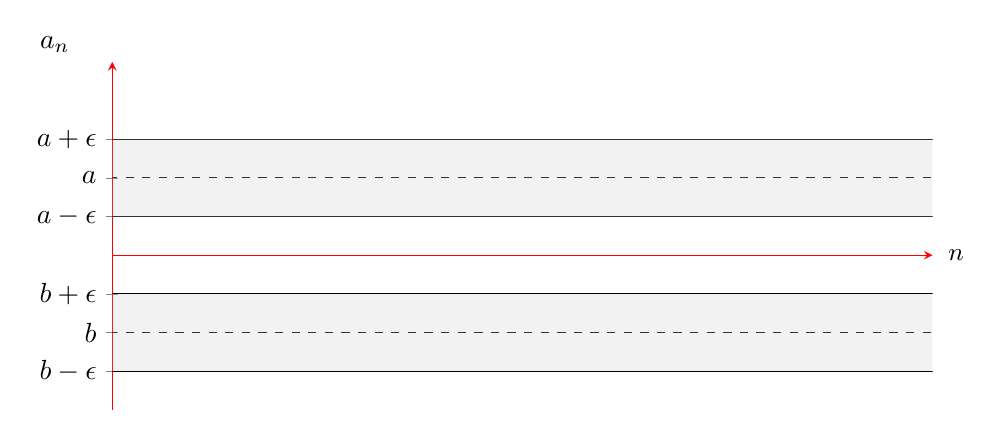
\begin{tikzpicture}
\begin{axis}[
 axis line style={red},
axis lines=middle,
     x label style={at={(axis description cs:1.05,0.4)}},
     y label style={at={(axis description cs:-0.1,1.1)}},
    xlabel={\small $n$},
    ylabel={$a_n$},
  ymin = -0.4,
  ymax = 0.5,
  xmin = 1,
  xmax = 10,
     ytick = {0.3, 0.2,0.1,-0.1,-0.2,-0.3},
   yticklabels={$a+\epsilon$,$a$, $a-\epsilon$,$b+\epsilon$, $b$, $b-\epsilon$},
   xtick = 0,
  width=12cm,height=6cm]
       \draw (axis cs:20,0.3) -- (axis cs:0,0.3); %a+e line
      \draw (axis cs:20,0.1) -- (axis cs:0,0.1); %a-e line
       \draw[dashed] (axis cs:20,0.2) -- (axis cs:0,0.2); %a line
         \fill[gray!40,nearly transparent] (axis cs:0,.1)-- (axis cs: 0,0.3) -- (axis cs: 10,0.3) -- (axis cs: 10,0.1) -- cycle;
         
          \draw(axis cs:20,-0.3) -- (axis cs:0,-0.3); %b+e line
      \draw (axis cs:20,-0.1) -- (axis cs:0,-0.1); %b-e line
       \draw[dashed]  (axis cs:20,-0.2) -- (axis cs:0,-0.2); %b line
         \fill[gray!40,nearly transparent] (axis cs:0,-.1)-- (axis cs: 0,-0.3) -- (axis cs: 10,-0.3) -- (axis cs: 10,-0.1) -- cycle;
  \end{axis}
\end{tikzpicture}
\end{center}

Eventually $a_n$ is in \emph{both} corridors. So if I choose $\epsilon$ sufficiently small so that corridors don't overlap to get a contradiction.

Set $\epsilon = \frac{|a-b|}{2} > 0$. Then $\exists N_a, N_b$ such that $\forall n \geq N_a,N_b$, we have 
\[|a_n - a| < \epsilon \text{ and } |a_n - b| < \epsilon\]
w.l.o.g. $a > b$. Then $a_n > a - \epsilon$ and $a_n < b$
\[\begin{aligned}
	&\implies b + \epsilon > a-\epsilon\\
	&\implies 2\epsilon > a-b = 2\epsilon~ \cont 
\end{aligned}\]
\end{proof}

\begin{clicker}
Prove $\frac{1}{n-2} \to 0$. Student Answer:
Fix $\epsilon >0$.
\begin{enumerate}
	\item We want $|\frac{1}{n-2} - 0| = \frac{1}{n-2} < \epsilon$
	\item $\implies n-2 > 1/\epsilon$
	\item $\implies n > 2 + 1/\epsilon$
	\item $\implies n > 1/\epsilon ~(*)$
	\item So take $N > 1/\epsilon$, then
	\item $\forall n \geq N$, $n > 1/\epsilon$ which is $(*)$
	\item So $\frac{1}{n-2} \to 0$
	\item (This is correct)
\end{enumerate}

\textbf{Answer:} (iv) is wrong. 
	
\end{clicker}


\begin{theorem}[Algebra of Limits]\label{thm1}
$a_n \to a$ and $b_n \to b$ then:\begin{enumerate}
\item $a_n+b_n \to a+b$
\item $a_nb_n \to ab$
\item $\frac{a_n}{b_n} \to \frac{a}{b} ~(b \neq 0)$
\end{enumerate}
\end{theorem}
\begin{proof}[Proof of (i)]
Fix any $\epsilon >0$. Then $\exists N_a \in \mathbb{N}$ such that $\forall n\geq N_a,~ |a_n	 - a| < \epsilon/2$ 

and $\exists N_b \in \mathbb{N}$ such that $\forall n \geq N_b,~ |b_n - b| < \epsilon/2$. Set $N =$ max$\{N_a,N_b\}$, so 
\[\begin{aligned}|(a_n + b_n) - (a+b)| &\leq |a_n -a| + |b_n -b| \\
	 &< \epsilon/2 + \epsilon/2 = \epsilon \qedhere
\end{aligned}\]
\end{proof}

\begin{proof}[Proof of (ii)]
\emph{Rough working:} 	
\[\begin{aligned}|a_nb_n -ab|  &= |(a_n -a)b - a_nb + a_nb_n|\\ 
&\leq |a_n-a||b| + |a_n|	|b_n-b|
\end{aligned}
\]

We can easily make $|a_n - a| < \epsilon/2$ if I take $|a_n - a| < \frac{\epsilon}{2|b|}$.

We need to show that $|a_n| < A$, so that I can take $|b_n - b| < \frac{\epsilon}{2A}$.\\

\begin{lemma}
If $a_n \to a$, then $(a_n)$ is bounded: $\exists A \in \RR \text{ s.t. }|a_n| < A,~\forall n$.
\end{lemma}
\begin{proof}[Proof of Lemma]~

\begin{center}
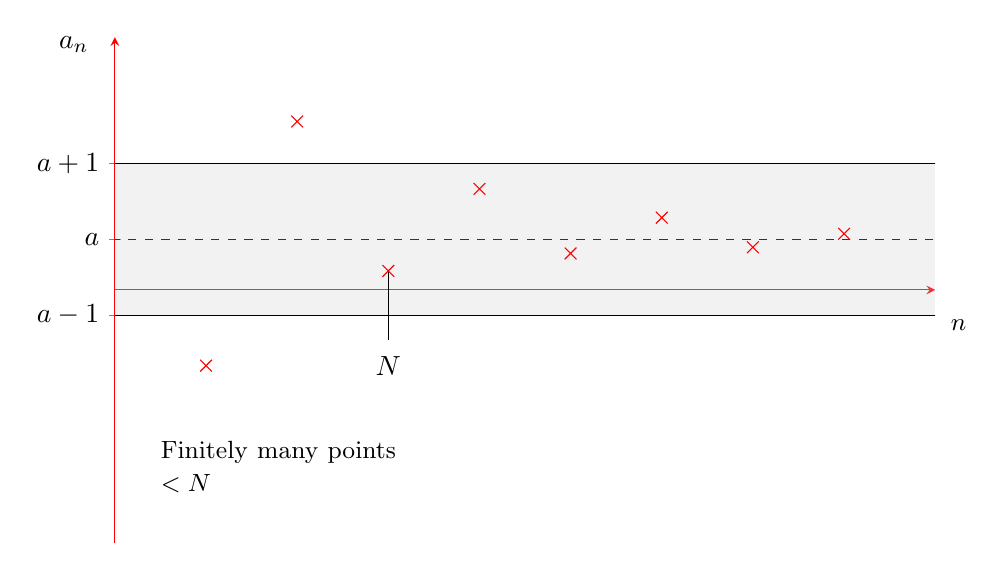
\begin{tikzpicture}
\begin{axis}[
 axis line style={red},
axis lines=middle,
     x label style={at={(axis description cs:1.05,0.4)}},
     y label style={at={(axis description cs:-0.08,1.02)}},
    xlabel={\small $n$},
    ylabel={$a_n$},
  ymin = -0.5,
  ymax = 0.5,
  xmin = 1,
  xmax = 10,
     ytick = {0.25, -0.05,0.1},
   yticklabels={$a+1$,$a-1$, $a$},
   xtick = 0,
  width=12cm,height=8cm]
   \addplot[samples at={3,5,7,9}, only marks, mark=x,  mark options={red}, mark size=3pt]{1/x};
    \addplot[samples at={2,4,6,8},only marks, mark options={red},mark=x,mark size=3pt]{-1/(x^2)+0.1};
       \draw (axis cs:20,0.25) -- (axis cs:0,0.25); %a+e line
      \draw (axis cs:20,-0.05) -- (axis cs:0,-0.05); %a-e line
       \draw[dashed] (axis cs:20,0.1) -- (axis cs:0,0.1); %a line
         \fill[gray!40,nearly transparent] (axis cs:0,-.05)-- (axis cs: 0,0.25) -- (axis cs: 10,0.25) -- (axis cs: 10,-0.05) -- cycle;
            \draw (axis cs:4,0.0375) -- (axis cs:4,-0.1) node at (axis cs:4,-0.15) {$N$};
                  \node[text width=3cm] at (axis cs:2.8,-0.35) {\small Finitely many points $<N$};
            
  \end{axis}
\end{tikzpicture}
\end{center}

Fix $\epsilon =1$. Then $\exists N \in \NN$ such that $\forall n \geq N,~|a_n - a| < 1 \implies |a_n| < 1 + |a|$. 

Then $(a_n)$ is bounded by max$\{a_1,a_2,\dots,a_{N-1},a+1\}$.
\end{proof}


Fix $\epsilon >0$. Then $\exists N_a$ such that $\forall n \geq N_a$, $|a_n - a| < \dfrac{\epsilon}{2(|b| + 1)}$ (we add $1$ in case $|b| = 0$)
and $\exists N_b$ such that $\forall n \geq N_b$, $|b_n - b| < \dfrac{\epsilon}{2A}$. 

Set $N = \text{max}(N_a,N_b)$. Then $\forall n \geq N$
\[\begin{aligned}|a_nb_n -ab| &\leq |a_n-a||b_n| + |b_n-b||a|\\ 
&< \frac{\epsilon}{2}\frac{|b|}{|b|+1} + A\frac{\epsilon}{2A}\\ 
& < \epsilon/2 + \epsilon/2 = \epsilon\qedhere	
\end{aligned}
\]
\end{proof}

See exercise sheet for proof of \ref{thm1}iii.\\

\begin{theorem}
If $(a_n)$ is bounded above \emph{and} monotonically increasing then $a_n$ is \emph{convergent}.
\end{theorem}

\emph{Idea:} 
\begin{center}
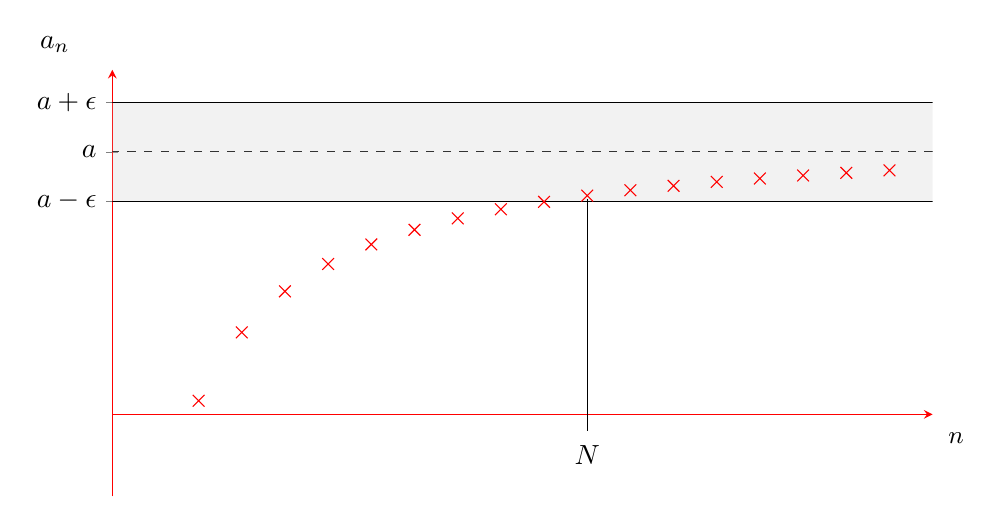
\begin{tikzpicture}
\begin{axis}[
 axis line style={red},
axis lines=middle,
     x label style={at={(axis description cs:1.05,0.1)}},
     y label style={at={(axis description cs:-0.1,1.1)}},
    xlabel={\small $n$},
    ylabel={$a_n$},
  ymin = -0.1,
  ymax = 0.42,
  xmin = 1,
  xmax = 20,
     ytick = {0.26,0.38,0.32},
   yticklabels={$a-\epsilon$,$a+\epsilon$,$a$},
   xtick = 0,
  width=12cm,height=7cm]
   \addplot[samples at={1,2,3,4,5,6,7,8,9,10,11,12,13,14,15,16,17,18,19}, only marks, mark=x,  mark options={red}, mark size=3pt]{0.35-1/x};
       \draw (axis cs:20,0.38) -- (axis cs:0,0.38);
              \draw (axis cs:20,0.26) -- (axis cs:0,0.26);
                     \draw[dashed] (axis cs:20,0.32) -- (axis cs:0,0.32);
         \fill[gray!40,nearly transparent] (axis cs:0,0.26)-- (axis cs: 0,0.38) -- (axis cs: 20,0.38) -- (axis cs: 20,0.26) -- cycle;
                     \draw (axis cs:12,0.262) -- (axis cs:12,-0.02) node at (axis cs:12,-0.05) {$N$};
  \end{axis}
\end{tikzpicture}
\end{center}
Eventually we get in the epsilon corridor (shaded area) because $a-\epsilon$ is \emph{not} an upper bound. We stay in there because monotonic and bounded by $a$.
\begin{proof}
Fix $\epsilon >0$. $a-\epsilon$ is \emph{not} an upper bound for $\{a_n : n \iN\}$ (because $a$ is the \emph{smallest} upper bound). So $\exists N \in \mathbb{N}$ such that $a_N > a-\epsilon$. Monotonic so $\forall n \geq N$ we have \[a\geq a_n\geq a_N > a-\epsilon \implies |a_n - a| < \epsilon\qedhere\]	
\end{proof}~

\begin{remark}\lecturemarker{6}{5 Oct}
 Now it's easier to handle things like $a_n = \dfrac{n^2 + 5}{n^3 - n + 6}$.

Dividing by $n^3$, we get $a_n = \dfrac{1/n + 5/n^3}{1 - 1/n^2 + 6/n^3}$.

 Use the fact that $1/n \to 0$ as $n \to \infty$ (Recall proof: $\forall \epsilon >0$, let $N_\epsilon  > 1/\epsilon$, then $n\geq N_{\epsilon} \implies n > 1/\epsilon \implies 1/n < \epsilon$), and the algebra of limits to deduce that 
\[a_n \to \dfrac{0 + 5.0^3}{1 - 0^2 + 6.0^3} = 0.\]
\end{remark}




\subsektion{Cauchy Sequences}
Gives a way of proving convergence \emph{without} knowing the limit.\\

\begin{definition}
	A sequence is Cauchy iff
	\[\forall \epsilon >0,~\exists N \in \mathbb{N} \text{ s.t. } \forall n,m \geq N,~ |a_n - a_m| < \epsilon\]
\end{definition}~

\begin{remark}
$m,n \geq N$ are arbitrary. It is not enough to say that $\forall \epsilon >0,~\exists N \in \NN$ such that $n \geq N \implies |a_n - a_{n+1}| < \epsilon$. See ex sheet. 	
\end{remark}

\begin{proposition}	
If $a_n \to a$ then $(a_n)$ is Cauchy. 
\end{proposition}
\begin{proof}
$a_n \to a\implies \forall \epsilon >0,~\exists N \text{ s.t. } n \geq N \implies |a_n - a| < \epsilon/2 ~(1)$


So $m \geq N \implies |a_m - a| < \epsilon /2 ~(2)$. So \[m,n \geq N \implies |a_n - a_m| \leq |a_n - a| + |a_m - a| < \underbrace{\epsilon/2}_{(1)} + \underbrace{\epsilon/2}_{(2)}=\epsilon\qedhere\]
\end{proof}

We want to prove converse: Cauchy $\implies$ Convergence.

We need a candidate for the limit $a$

\begin{center}
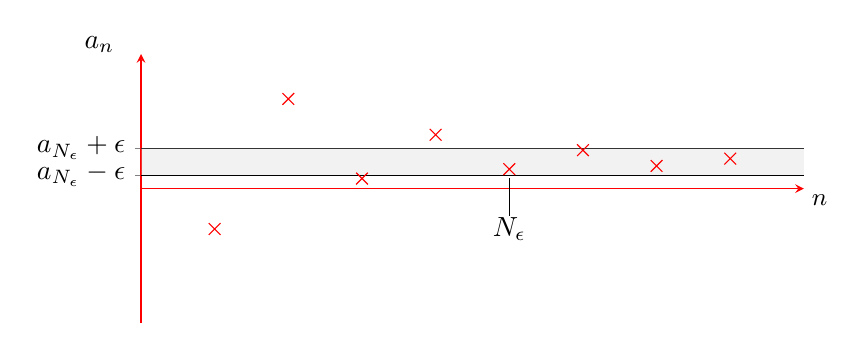
\begin{tikzpicture}
\begin{axis}[
 axis line style={red},
axis lines=middle,
     x label style={at={(axis description cs:1.05,0.4)}},
     y label style={at={(axis description cs:-0.1,1.1)}},
    xlabel={\small $n$},
    ylabel={$a_n$},
  ymin = -0.5,
  ymax = 0.5,
  xmin = 1,
  xmax = 10,
     ytick = {0.15, 0.05},
   yticklabels={$a_{N_{\epsilon}}+\epsilon$,$a_{N_{\epsilon}}-\epsilon$},
   xtick = 0,
  width=10cm,height=5cm]
   \addplot[samples at={3,5,7,9}, only marks, mark=x,  mark options={red}, mark size=3pt]{1/x};
    \addplot[samples at={2,4,6,8},only marks, mark options={red},mark=x,mark size=3pt]{-1/(x^2)+0.1};
       \draw (axis cs:20,0.15) -- (axis cs:0,0.15); %a+e line
      \draw (axis cs:20,0.05) -- (axis cs:0,0.05); %a-e line
       %\draw[dashed] (axis cs:20,0.1) -- (axis cs:0,0.1); %a line
         \fill[gray!40,nearly transparent] (axis cs:0,.05)-- (axis cs: 0,0.15) -- (axis cs: 10,0.15) -- (axis cs: 10,0.05) -- cycle;
            \draw (axis cs:6,0.04) -- (axis cs:6,-0.1) node at (axis cs:6,-0.15) {$N_\epsilon$};
     
            
  \end{axis}
\end{tikzpicture}
\end{center}

We will produce an auxiliary sequence which is \emph{monotonic} (+ bounded) $\implies$ convergence. $b_n:= \mathrm{sup}\{a_i : i \geq n\}$. Then picture shows that $b_{N_{\epsilon}} \in (a_{N_{\epsilon}} - \epsilon, a_{N_{\epsilon}} + \epsilon]$ and $b_n$'s are monotonically \emph{decreasing} because $b_{n+1} = \mathrm{sup}\{a_i : i \geq n+1\}$, a subset of $\{a_i : i \geq n\}$. 

So $b_n$s converge to $\mathrm{inf}\{b_n: n \iN\}$. We will show that $a_n$'s converge to same number, $a$, using Cauchy condition. 

\begin{lemma}
$(a_n)$ is Cauchy $\implies (a_n)$ is bounded
\end{lemma}

\begin{proof}
Pick $\epsilon =1$, then $\exists N$ such that $\forall n,m \geq N$, $|a_n - a_m|  < 1$. In particular $|a_n| < 1 + |a_N|~\forall n \geq N$ (take $m = N$), so 
\[|a_n| \leq \mathrm{max}\{|a_1|,|a_2|,\dots|a_{N-1}|,1+|a_N|\}~\forall N \iN\qedhere\]	
\end{proof}


\begin{theorem}
$(a_n)$ is a Cauchy sequence of real numbers $\implies a_n$ convergent. 
\end{theorem}

\begin{corollary}
$(a_n)$ Cauchy $\iff (a_n)$ convergent. (Ex: Show not true in $\QQ$!) 	
\end{corollary}

\begin{proof}
$(a_n)$ Cauchy $\implies$ bounded. So we can define $b_n = \mathrm{sup}\{a_i : i \geq n\}$. Then define $a = \mathrm{inf}\{b_n : n \iN\}$ and we prove that $a_n \to a$.

Fix $\epsilon > 0$. $\exists N \iN$ s.t. $n,m \geq N  \implies |a_n - a_m| < \epsilon/2 \iff a_n - \epsilon/2 < a_m < a_n + \epsilon /2$.
Take supremum over all $m \geq i \geq N$
\[\begin{aligned}
\implies a_n - \epsilon/2 &< \mathrm{sup}	\{a_m: m \geq i\} \leq a_n + \epsilon/2\\
\text{ i.e. } a_n - \epsilon/2 &< b_i \leq a_n + \epsilon/2\\
\implies a_n - \epsilon/2 &\leq \equalto{\mathrm{inf}	\{b_i: i \geq N\}}{a} \leq a_n + \epsilon/2\\
\iff |a-a_n| &\leq \epsilon/2 < \epsilon \quad \forall n \geq N.\end{aligned}\]
(We used: $S \subseteq \RR$ is bounded satisfying $x < M~\forall x \in S$. Then $\mathrm{sup}S \leq M$.)
\end{proof}

\pagebreak
\lecturemarker{7}{5 Oct}

\begin{example}
Prove that if $\left|a_{n+1}/a_n\right|\to L$, $L < 1$, then $a_n \to 0$	

\emph{Idea:} $a_N \approx c.L^n$ for $n >> 0$, $L<1 \implies a_n \to 0$. 

To turn this in to a proof, we want $\left|a_{n+1}/a_n\right|$ to be less than $\alpha <1$! We can't take $\alpha = L$! We can take $\alpha = L + \epsilon$ (because $\left|a_{n+1}/a_n\right|$ is \emph{not} equal to $L$; it just tends to it). So we need $L + \epsilon < 1$, so take $\epsilon = \frac{1-L}{2}$.

\begin{proof}
Fix $\epsilon = \frac{1-L}{2} > 0$ (because $L < 1$). $\exists N \iN$ such that $\forall n \geq N$
\[\left|\frac{a_{n+1}}{a_n} - L\right| < \epsilon \implies \left|\frac{a_{n+1}}{a_n}\right| < L + \epsilon = L + \frac{1-L}{2} = \frac{1+L}{2} < 1\]
So inductively we find that
\[|a_{N+k}| \leq \frac{1+L}{2} |a_{N+k-1}| \leq \left(\frac{1+L}{2}\right)^2 |a_{N+k-2}| \leq \dots \leq \left(\frac{1+L}{2}\right)^k |a_{N}| ~(*)\]
[Ex sheet: $\alpha^k \to 0$ as $k \to \infty$ if $|\alpha| < 1$]

Applying this to $\alpha = \frac{1+L}{2} < 1$. $\exists M > 0$ s.t. $\forall m \geq M$

\[\left(\frac{1+L}{2}\right)^M < \frac{\epsilon}{1 + |a_N|}\]
(as before we add $1$ in denominator in case $|a_N| = 0$)

So by $(*)$ we have $|a_{N+m}| < \dfrac{\epsilon|a_N|}{1 + |a_N|} < \epsilon~\forall m \geq M$. Rewriting this: 
\[\forall n \geq N+M,~ |a_n| < \epsilon\qedhere\]
\end{proof}
\end{example}~

\subsektion{Subsequences}

\begin{definition}
A \emph{subsequence} of $(a_n)$ is a new sequence $b_i = a_{n(i)}~ \forall i \iN$ where $n(1) < n(2) < \dots < n(i) < \dots ~\forall i \implies n(i) \geq i$ (Ex: prove this by induction)

[Formally $n(i)$ is a function $\NN \to \NN$ with $i \mapsto n(i)$ which is strictly monotonically increasing.] ``Just go down the sequence faster, missing some terms out''
\end{definition}~

\begin{example}
$a_n = (-1)^n$ has subsequences:
\begin{itemize}
	\item $b_n = a_{2n}$, so $b_n = 1~\forall n \implies b_n \to 1$
	\item $c_n = a_{2n+1}$, so $c_n = -1~\forall n \implies c_n \to -1$
	\item $d_n = a_{3n}$, so $d_n = (-1)^n (=a_n!)$ doesn't converge. 
	\item $e_n = a_{n+17}$, so $e_n = (-1)^{n+1} = -a_n$ doesn't converge.
\end{itemize}

\end{example}


Next we work up to 


\begin{theorem}[Bolzano-Weierstrass]
If $(a_n)$ is a \emph{bounded} sequence of real numbers then it has a \emph{convergent subsequence}.
\end{theorem}


\begin{proof}[Cheap proof]

Use ``peak points'' of $(a_n)$
\begin{center}
\begin{tikzpicture}
\begin{axis}[
 axis line style={red},
axis lines=middle,
     x label style={at={(axis description cs:1.05,0)}},
     y label style={at={(axis description cs:-0.05,1.1)}},
    xlabel={\small $n$},
    ylabel={$a_n$},
  ymin = 0,
  ymax = 8,
  xmin = 1,
  xmax = 12,
    ytick = 0,
   xtick = 0,
  width=10cm,height=6cm]
\addplot[color=red,mark=x] coordinates {
		(2,1)
		(3,2)
		(4,7)
		(5,3.4)
		(6,4)
		(7,2)
		(8,5.3)
		(9,3.5)
		(10,2.8)
	};
          \draw[->] (axis cs:4,7) -- (axis cs:12,7);
          \draw[->] (axis cs:8,5.3) -- (axis cs:12,5.3);
        \node at (axis cs: 4,7.4) {\small peak};
        \node at (axis cs: 8,5.7) {\small peak};
  \end{axis}
\end{tikzpicture}
\end{center}

We say that $a_j$ is a \emph{peak point} iff $a_k < a_j ~\forall k > j$.
Either
\begin{enumerate}
	\item $(a_n)$ has a finite no. of peak points
	\item $(a_n)$ has an infinite no. of peak points
\end{enumerate}

\textbf{Case (i):} Pick $n(1) \geq \mathrm{max}(j_1,\dots,j_k)$ where $a_{j1},\dots,a_{jk}$ are the finite no. of peak points. 

``Go beyond the (finitely many) peak points''.

$a_{n(1)}$ is not a peak point $\implies \exists n(2) > n(1)$ s.t. $a_{n(2)} \geq a_{n(1)}$. 

Similarly $a_{n(2)}$ not a peak point $\implies \exists n(3) > n(2)$ s.t. $a_{n(3)} \geq a_{n(2)}$.

Recursively no peak pints beyond $n(1) \implies$ we get $n(i) > n(i-1) > \dots > n(1)$ s.t. $a_{n(i)} \geq a_{n(i-1)}~\forall i$.

\begin{center}
\begin{tikzpicture}
\begin{axis}[
 axis line style={red},
axis lines=middle,
     x label style={at={(axis description cs:1.05,0)}},
     y label style={at={(axis description cs:-0.05,1.1)}},
    xlabel={\small $n$},
    ylabel={$a_n$},
  ymin = 0,
  ymax = 8,
  xmin = 1,
  xmax = 13,
     ytick = 0,
   xtick = {4,8,11},
   xticklabels = {$n(1)$,$n(2)$,$n(3)$},
  width=10cm,height=7cm]
\addplot[color=red,mark=x] coordinates {
		(4,2.2)
		(5,2)
		(6,1.2)
		(7,3)
		(8,4.5)
		(9,2.4)
		(10,3.6)
		(11,6)
		(12,5.5)
	};
	\addplot[only marks, color=red,mark=o] coordinates {
		(4,2.2)
		(8,4.5)
		(11,6)
	};
        \draw (axis cs:4,6) -- (axis cs:4,-0.1);
  \end{axis}
\end{tikzpicture}
\end{center}

i.e. $a_{n(i)}$ is a monotonically increasing subsequence of $a_n$. $(a_n)_{n\geq 1}$ bounded $\implies (a_{n(i)})_{i\geq 1}$ is bounded $\implies a_{n(i)}$ is convergent (to $\mathrm{sup}\{a_{n(i)} : i \iN\}$.


\textbf{Case (ii):} $\exists$ infinitely many peak points. Call these peak points $a_{n(1)}, a_{n(2)},\dots$ where $n(1) > n(2) > \dots$

\begin{center}
\begin{tikzpicture}
\begin{axis}[
 axis line style={red},
axis lines=middle,
     x label style={at={(axis description cs:1.05,0)}},
     y label style={at={(axis description cs:-0.05,1.1)}},
    xlabel={\small $n$},
    ylabel={$a_n$},
  ymin = 0,
  ymax = 8,
  xmin = 1,
  xmax = 13,
     ytick = 0,
   xtick = {4,8,11},
   xticklabels = {$n(1)$,$n(2)$,$n(3)$},
  width=10cm,height=6cm]
\addplot[color=red,mark=x] coordinates {
		(12,1)
		(11,2)
		(10,1.2)
		(9,3)
		(8,4.5)
		(7,2.4)
		(6,3.6)
		(5,3.2)
		(4,6)
	};
	\addplot[only marks, color=red,mark=o] coordinates {
		(11,2)
		(8,4.5)
		(4,6)
	};
        \draw (axis cs:4,6) -- (axis cs:4,-0.1);
  \end{axis}
\end{tikzpicture}
\end{center}

$a_{n(i+1)} \leq a_{n(i)}$ because $n(i+1) > n(i)$ and $a_{n(i)}$ is a peak point $\implies (a_{n(i)})_{i\geq 1}$ is monotonically decreasing and bounded $\implies$ convergent (to $\mathrm{inf}\{a_{n(i)} : i \iN\}$.
\end{proof}




\begin{proposition}\label{prop1}\lecturemarker{8}{5 Oct}
If $a_n \to a$ as $n\to \infty$ then any subsequence $a_{n(i)} \to a$ as $i \to \infty$	
\end{proposition}

\begin{proof}
\[\forall \epsilon >0,~\exists N \iN \text{ s.t. } \forall n \geq N,~|a_n - a| < \epsilon ~(*)\]	
But $\forall i \geq N$, then $n(i) \geq i \geq N \implies$ by $(*),~|a_{n(i)} - a| < \epsilon$.
\end{proof}

This gives us another proof that $(-1)^n$ is not convergent, because if $(-1)^n \to a$, then by Prop \ref{prop1}, $(-1)^{2n} \to a$ and $(-1)^{2n+1} \to a \implies a = 1$ and $a = 1,~\cont$\\

We also get another proof of ``Cauchy $\implies$ convergence'' using BW (Bolzano-Weierstrass). If $a_n$ is Cauchy ($\forall \epsilon >0 ~\exists N \iN$ s.t. $\forall n,m \geq N~|a_n -a_m | < \epsilon$), then $a_n$ is convergent $(\exists a$ s.t. $a_n \to a$)

\begin{proof}
	We know that $a_n$ is bounded (by $\mathrm{max}\{|a_1|,|a_2|,\dots,|a_{N-1}|,|a_N| + 1)\}$. So by BW, $\exists$ a convergent subsequence $a_{n(i)},~i \geq 1$ s.t. $a_{n(i}) \to a$ as $i \to \infty$ for some $a \iR$. 
	
	So fix $\epsilon >0$. We have:
	\begin{enumerate}
	\item $\exists N_1$ s.t. $\forall n,m \geq N_1,~|a_n - a_m| < \epsilon$
	\item $\exists N_2$ s.t. $\forall i \geq N_2,~|a_{n(i)} -a | < \epsilon$	
	\end{enumerate}

\begin{center}
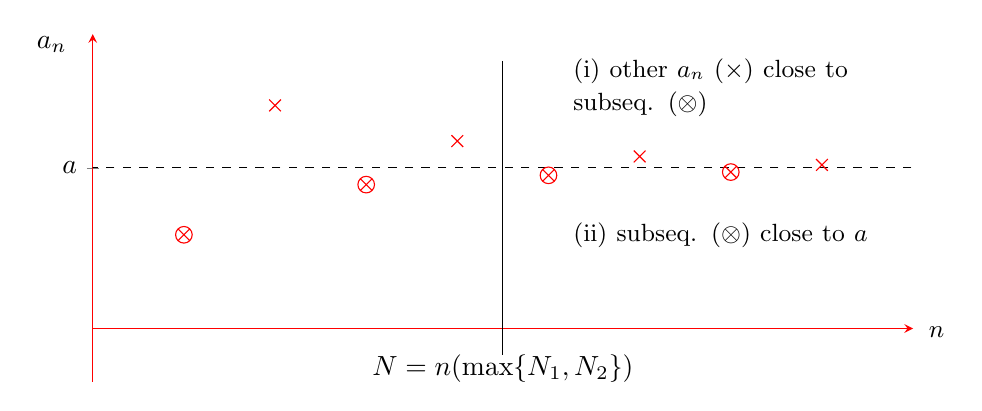
\begin{tikzpicture}
\begin{axis}[
 axis line style={red},
axis lines=middle,
     x label style={at={(axis description cs:1.05,0.1)}},
     y label style={at={(axis description cs:-0.08,1.02)}},
    xlabel={\small $n$},
    ylabel={$a_n$},
  ymin =-0.2,
  ymax = 1.1,
  xmin = 1,
  xmax = 10,
     ytick = {0.6},
   yticklabels={$a$},
   xtick = 0,
  width=12cm,height=6cm]
   \addplot[samples at={3,5,7,9}, only marks, mark=x,  mark options={red}, mark size=3pt]{1/x+0.5};
    \addplot[samples at={2,4,6,8},only marks, mark options={red},mark=otimes,mark size=3pt]{-1/(x^2)+0.6};
       \draw[dashed] (axis cs:20,0.6) -- (axis cs:0,0.6); %a line
            \draw (axis cs:5.5,1) -- (axis cs:5.5,-0.1) node  at (axis cs:5.5,-0.15) {$N =n(\mathrm{max}\{N_1,N_2\})$}; %N line
                  \node[text width=4cm] at (axis cs:8,0.9) {\small (i) other $a_n$ ($\times$) close to subseq. ($\otimes$)};
          \node[text width=4cm] at (axis cs:8,0.35) {\small (ii) subseq. ($\otimes$) close to $a$};
            
  \end{axis}
\end{tikzpicture}
\end{center}

Set $N = n(\mathrm{max}\{N_1,N_2\}) \geq \mathrm{max}\{N_1,N_2\} \geq N_1$. Then $\forall n \geq N$ we have
\[\begin{aligned}|a_n - a| &= |(a_n - a_N) + (a_N - a)| \\
&\leq |a_n - a_N| + |a_N - a|\\
 &< \epsilon + \epsilon = 2\epsilon	
\end{aligned}\]\end{proof}\vspace*{5pt}


\textbf{Aside:} Fix $c >0$. Then $a_n \to a$ iff 
\[\boxed{\forall \epsilon >0,~\exists N_{\epsilon} \iN \text{ s.t. } n \geq N_\epsilon \implies |a_n - a| < c\epsilon (*)}\]
Ex: Show $\implies$

\begin{proof}[Proof $\impliedby$] Fix $\epsilon >0$. Set $e' = \epsilon/c >0$. Then $(*) \implies $
\[\exists N_\epsilon \iN \text{ s.t. } n \geq N_\epsilon \implies |a_n - a| < c\epsilon' = \epsilon\qedhere\]
\end{proof}

\textbf{Beware!} Do not let $c$ depend on $\epsilon$ (Nor $N!$), e.g. if we let $c = \frac{1}{\epsilon}$ then $(*)$ becomes $\forall \epsilon >0,~\exists N \iN$ s.t. $\forall n \geq N,~|a_n - a| < 1$ and $a_n = \frac{1}{2} \forall n,~ a = 0$ satisfies this!\\

We can also go the other way round: Cauchy theorem $\implies$ BW. 

\begin{proof}[Proof 2 of BW]



Take a bounded sequence $(a_n)$. We want to find a convergent subsequence. 

Given $a_n \in [-R,R]~ \forall n$, repeatedly subdivide to make this interval smaller. So either
\begin{enumerate}
\item $\exists$ infinite number of $a_n$'s in $[-R,0]$
\item $\exists$ infinite number of $a_n$'s in $[0,R]$
\end{enumerate}

Pick one of these intervals with inifnite number of $a_n$'s; call it $[A_1,B_1]$, length $2R/2$. 

Now subdivide again; call $[A_2,B_2]$ one of the intervals $[A_1,\frac{A_1+B_1}{2}]$ or $[\frac{A_1+B_1}{2},B_1]$ with infinitely many $a_n$'s in it with length $2R/2^2$ etc. 

We get a sequence of intervals $[A_n,B_n]$ of length $2R/2^n$ each containing an infinite number of $a_n$s which are nested: $[A_{k+1},B_{k+1}] \subseteq [A_k,B_k]$


Now we use a \emph{diagonal argument}. Let $b_i = a_{n(i)}$ be an elements of the sequence in $[A_i,B_i]$ s.t. $n(i) > n(i-1)$. (This is possible because $\exists$ infinite no. of elements of sequence in $[A_i,B_i]$. 

 \textbf{Claim:} $b_i = a_{n(i)}$ is convergent.

Fix $\epsilon >0$. Take $N_{\epsilon} > \frac{2R}{\epsilon}$, so that $\frac{2R}{2^{N_{\epsilon}}} < \frac{2R}{N_{\epsilon}} < \epsilon$. Then $\forall i, j \geq N_{\epsilon}$ we have
\[|b_i - b_j| < \frac{2R}{2^{N_{\epsilon}}} < \epsilon\]
beacause $b_i,b_j \in [A_{N_{\epsilon}},B_{N_{\epsilon}}] \implies (b_i)$ Cauchy $\implies$ convergent.
	\end{proof}\vspace*{5pt}
	

